\documentclass[tikz,dvipdfmx]{standalone}

\usepackage{amsmath, amssymb, amsthm, mathrsfs, amsfonts, dsfont}
\usepackage{mathtools}

\usetikzlibrary{3d}

\definecolor{cA}{HTML}{0072BD}
\definecolor{cB}{HTML}{EDB120}
\definecolor{cC}{HTML}{77AC30}
\definecolor{cD}{HTML}{D95319}

\begin{document}

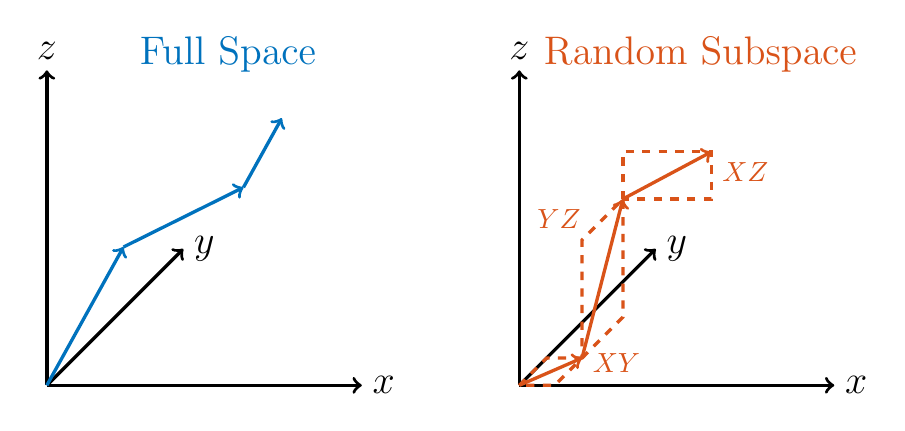
\begin{tikzpicture}
  \node[cA] at (-3+2.3,4.2) {\Large{Full Space}};
  \begin{scope}[shift={(-3,0)}]
    \draw[->, very thick] (0,0,0) -- (4,0,0) node[anchor=west] {\Large$x$};
    \draw[->, very thick] (0,0,0) -- (0,4,0) node[anchor=south] {\Large$z$};
    \draw[->, very thick] (0,0,0) -- (0,0,-4.5) node[anchor=west] {\Large$y$};
    \coordinate (O) at (1.1*   0, 1.*  0, 1.1*  0);
    \coordinate (A) at (1.1* 0.5, 1.*4/3, 1.1* -1);
    \coordinate (B) at (1.1* 1.5, 1.*5/3, 1.1* -2);
    \coordinate (C) at (1.1*1.75, 1.*7/3, 1.1*-2.5);
    \draw[->,very thick, cA] (O)--(A);
    \draw[->,very thick, cA] (A)--(B);
    \draw[->,very thick, cA] (B)--(C);
  \end{scope}

  \node[cD] at (+3+2.3,4.2) {\Large{Random Subspace}};
  \begin{scope}[shift={(+3,0)}]
    \draw[->, very thick] (0,0,0) -- (4,0,0) node[anchor=west] {\Large$x$};
    \draw[->, very thick] (0,0,0) -- (0,4,0) node[anchor=south] {\Large$z$};
    \draw[->, very thick] (0,0,0) -- (0,0,-4.5) node[anchor=west] {\Large$y$};
    \coordinate (O) at (0.9*0   , 0.9*  0, 0.9*   0);
    \coordinate (A) at (0.9*0.5 , 0.9*  0, 0.9*  -1);
    \coordinate (B) at (0.9*0.5 , 0.9*5/3, 0.9*-2.5);
    \coordinate (C) at (0.9*1.75, 0.9*7/3, 0.9*-2.5);
    \draw[->,very thick, cD] (O)--(A);
    \draw[->,very thick, cD] (A)--(B);
    \draw[->,very thick, cD] (B)--(C);
    \draw[canvas is xz plane at y=0   ,very thick, dashed, cD] (O) rectangle (A) node[anchor=north west, shift={(0,0.2)}] {$XY$};
    \draw[canvas is yz plane at x=0.5 ,very thick, dashed, cD] (A) rectangle (B) node[anchor=north east, shift={(-0.4,0)}] {$YZ$};
    \draw[canvas is xy plane at z=-2.5,very thick, dashed, cD] (B) rectangle (C) node[anchor=north west] {$XZ$};
  \end{scope}
\end{tikzpicture}

\end{document}
